\documentclass[12pt]{article}
\usepackage[utf8]{inputenc}
%\usepackage[portuguese]{babel}
\usepackage{amsmath,amsfonts,amssymb}
\usepackage{graphicx}
\usepackage{makeidx}
\usepackage{graphicx}
\usepackage{lmodern}
\usepackage{multicol}
\usepackage{booktabs}
\usepackage{fancyhdr}
\usepackage{hyperref}
\usepackage[usenames]{color}


\usepackage{Sweave}
\begin{document}
\Sconcordance{concordance:KDE.tex:KDE.Rnw:%
1 15 1 1 0 51 1 1 2 1 0 1 12 13 0 1 2 4 1 1 21 23 0 1 2 3 1 1 30 13 0 1 %
1 2 0 1 1 3 0 1 2 4 1 1 34 1 2 5 1 1 34 1 2 5 1 1 7 1 2 5 1 1 9 1 2 16 %
1}

\pagestyle{fancy}
\fancyhf{}
\renewcommand{\headrulewidth}{0.4pt}
\fancyfoot[C]{\thepage}
\renewcommand{\footrulewidth}{0.4pt}
\fancyfoot[C]{\thepage}
\title{\LARGE \bf
 Exercício 9 - Estimação de densidades utilizando KDE}
\author{ Rodrigo Machado Fonseca - 2017002253}
\thispagestyle{fancy}
\fancyhead[C]{Introdução ao Reconhecimento de Padrões - UFMG \\ Belo Horizonte - \today}
\maketitle
\thispagestyle{fancy}

%%%%%%%%%%%%%%%%%%%%%%%%%%%%%%%%%%%%%%%%%%%%%%%%%%%%%%%%%%%%%%%%%%%%%%%%%%%%%%%%%%%%%%%%%
\section{Introdução}
   \par Neste trabalho iremos implementar o algoritmo KDE (\textit{Kernel  density estimation}) \ref{KDE}. Em seguida, iremos utilizá-lo para classificar um conjunto de amostras.
   
\section{KDE}
  \label{KDE}
  \par A maioria dos problemas que lidamos não são bem comportados. Onde os modelos normais não se aplicam é possível utilizar modelos não-paramétricos, que é o caso do KDE.
  
  \par O KDE vai realizar a estimativa, por meio da superposição de funções de densidade em cada ponto da amostra.
  
  \par Neste experimento utilizaremos a função de densidade normal como função de kernel:
  
  \begin{equation}
  p(x) = \frac{1}{N}\sum_{i=1}^{N}\frac{1}{h}K(\frac{x-x_i}{h})
  \end{equation}
  
  \begin{equation}
  K(\frac{x-x_i}{h}) = \frac{1}{\sqrt{2\pi}}\cdot exp(-0.5(\frac{x-x_i}{h})^2)
  \end{equation}
  
  \par Para calcular o valor \textit{h} utilizaremos a regra  Silvermann:
  
  \begin{equation}
  h \approx 1.06\sigma N^{-0.2},
  \end{equation}
  
  \par onde $\sigma$ é o desvio padrão da classe e N é o número de amostras.
  
  \par Para o problema multivariado  utilizaremos a seguinte fórmula:
  
  \begin{equation}
  p(x_i) = \frac{1}{N(\sqrt{2\pi h})^N}\Sigma_{j = 1}^{N}e^{-\frac{(x_i - x_j)^2}{2h^2}}
  \label{px}
  \end{equation}
  
  \par a função a seguir condensa o que foi discutido nesta seção.
\begin{Schunk}
\begin{Sinput}
> rm(list=ls())
> pdfKDE <- function(xi, N, x)
+ {
+   sum <- 0
+   h <- 1.06 * sd(x) * N^(-1/5)
+   for (i in 1:N)
+   {
+     sum <- sum + exp(-(1/(2*h^2) * (t(x[i, ] - xi) %*% (x[i, ] - xi))))
+   }
+   p <- (1/(N * (sqrt(2 * pi * h))^N)) * sum
+   return (p)
+ }
\end{Sinput}
\end{Schunk}

\section{Metodologia}

  \par Inicialmente, carregamos os dados da base \textit{mlbench.spirals}. Em sequência, foi necessário separar as amostras em treinamento e teste utilizando a técnica de validação cruzada com 10 folds. O processo de treinamento e teste será repetido 10 vezes, de forma que a cada vez utilizaremos um dos 10 folds para o teste e os outros 9 para treinamento. Para cada par treinamento e teste utilizaremos o classificador de bayes.

\begin{Schunk}
\begin{Sinput}
> bayes_classifier <- function(x_train, y_train, x_test){
+   pC1 = (nrow(x_train[y_train == 1, ])) / nrow(x_train)
+   pC2 = 1-pC1
+   c1 = x_train[y_train == 0, ]
+   c2 = x_train[y_train == 1, ]
+   y_hat <- c()
+   for(i in 1:nrow(x_test)){
+     p1 <- pdfKDE(x_test[i, ], nrow(c1),
+                  c1)
+     p2 <- pdfKDE(x_test[i, ], nrow(c2),
+                  c2)
+     if(p1*pC1/(p2*pC2) >= 1){
+       y_hat <-c(y_hat, 0)
+     }
+     else{
+       y_hat <- c(y_hat, 1)
+     }
+   }
+   return(y_hat)
+ }
\end{Sinput}
\end{Schunk}

\section{Resultados}

  \par A seguir estão apresentados os valores da acurácia obtido para cada iteração, o desvio padrão das acurácias e a média das acurácias, respectivamente. 
\begin{Schunk}
\begin{Soutput}
      [,1]
 [1,] 1.00
 [2,] 0.90
 [3,] 1.00
 [4,] 0.90
 [5,] 0.80
 [6,] 1.00
 [7,] 0.90
 [8,] 0.75
 [9,] 1.00
[10,] 0.90
\end{Soutput}
\begin{Soutput}
[1] 0.08834906
\end{Soutput}
\begin{Soutput}
[1] 0.915
\end{Soutput}
\end{Schunk}

  \par Para o fold 1 iremos plotar os dados de testes no espaço de verossimilhanças, a superfície de densidade de probabilidade, o conjunto de amostras antes do treinamento e após o treinamento, respectivamente.

\begin{figure}[h]
\centering
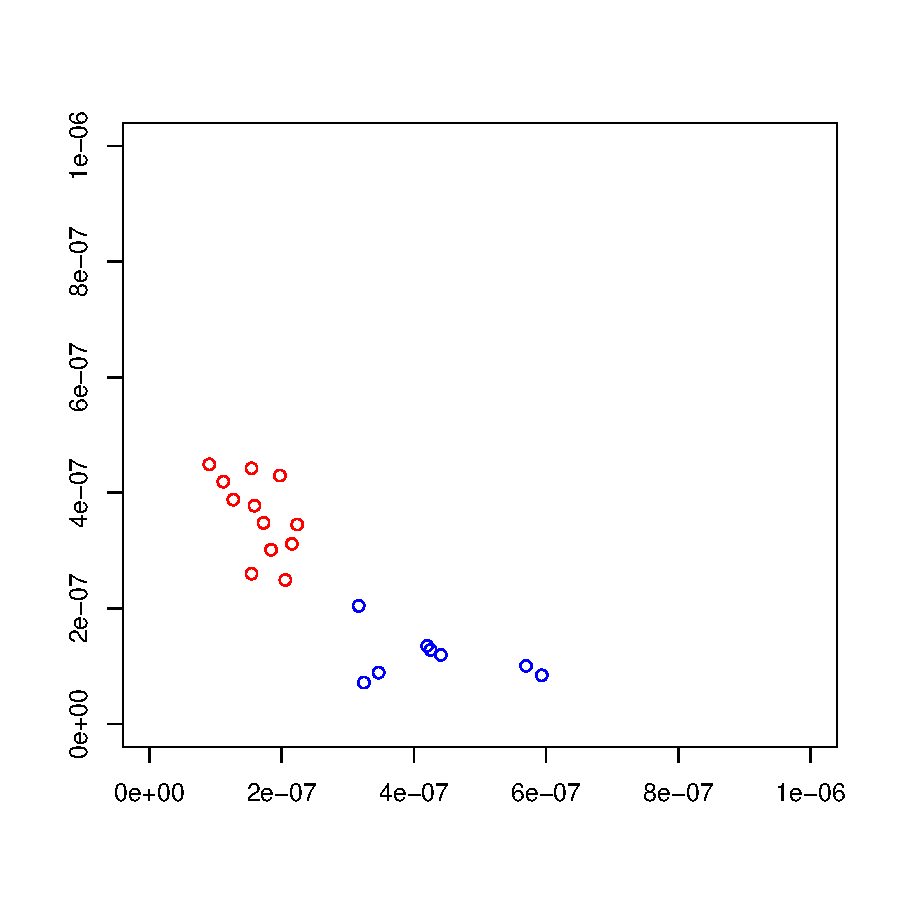
\includegraphics{KDE-004}
\caption{Dados de teste no espaço de verossimilhanças para o fold 1}
\label{8}
\end{figure}

\begin{figure}[h]
\centering
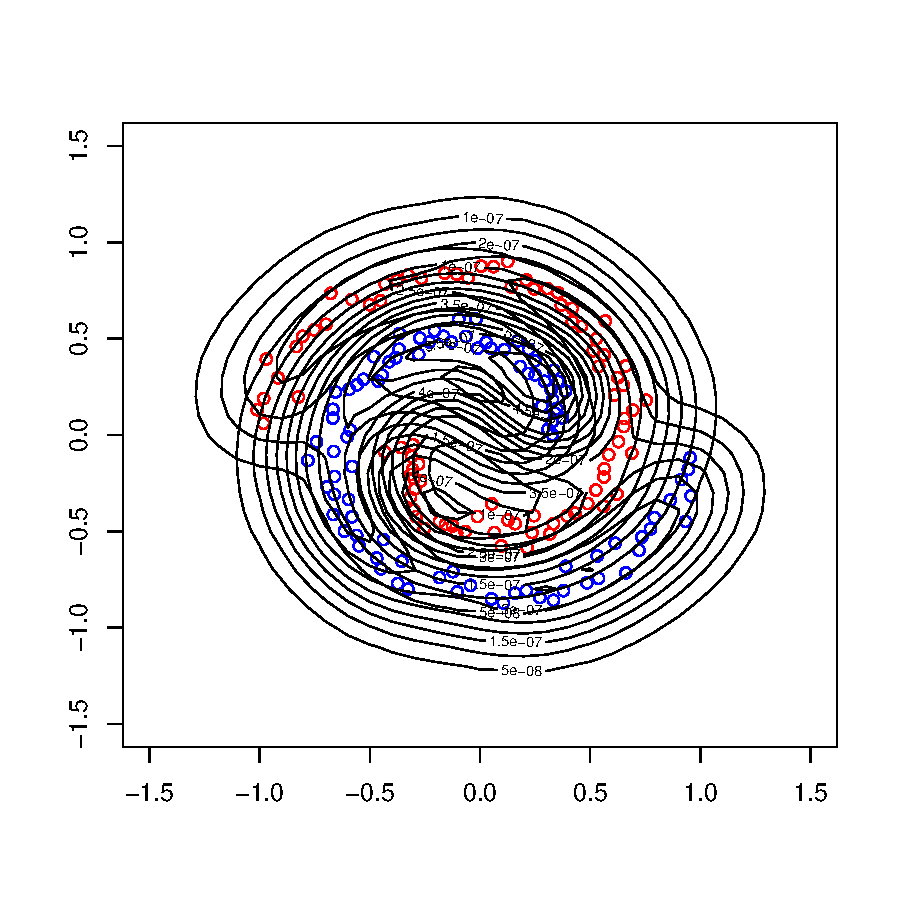
\includegraphics{KDE-005}
\caption{Superfície de densidade de probabilidade para o fold 1.}
\label{9}
\end{figure}

\begin{figure}[h]
\centering
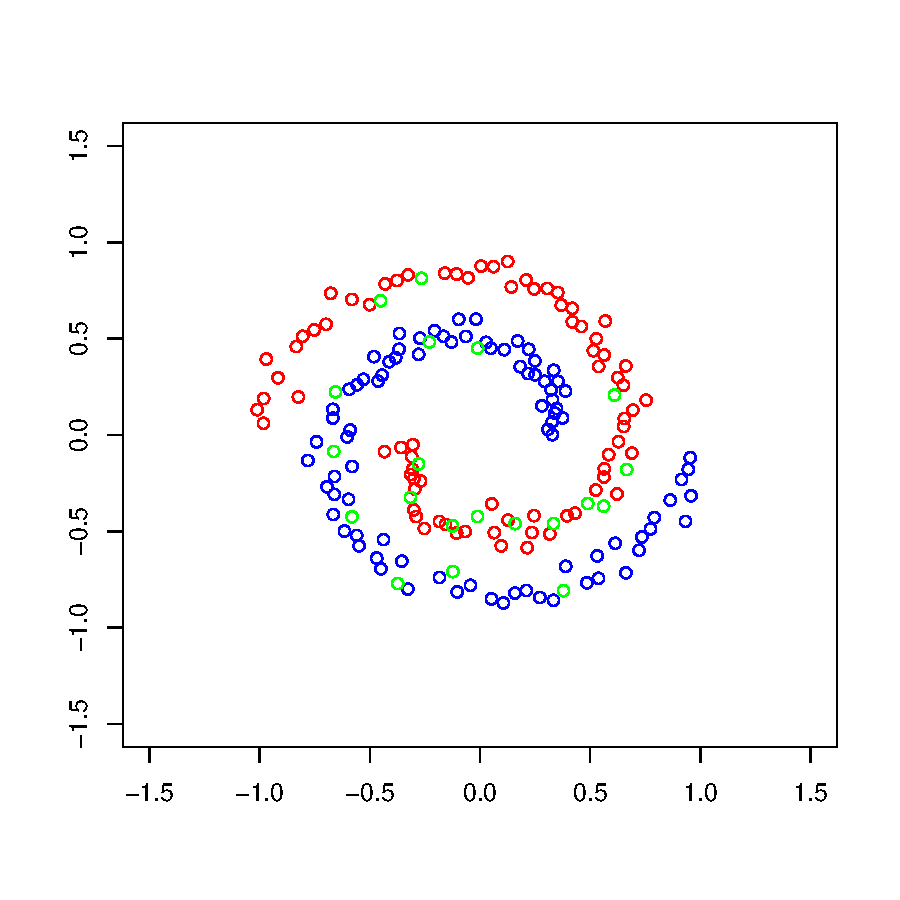
\includegraphics{KDE-006}
\caption{Amostras antes da classificação para o fold 1.}
\label{10}
\end{figure}

\begin{figure}[h]
\centering
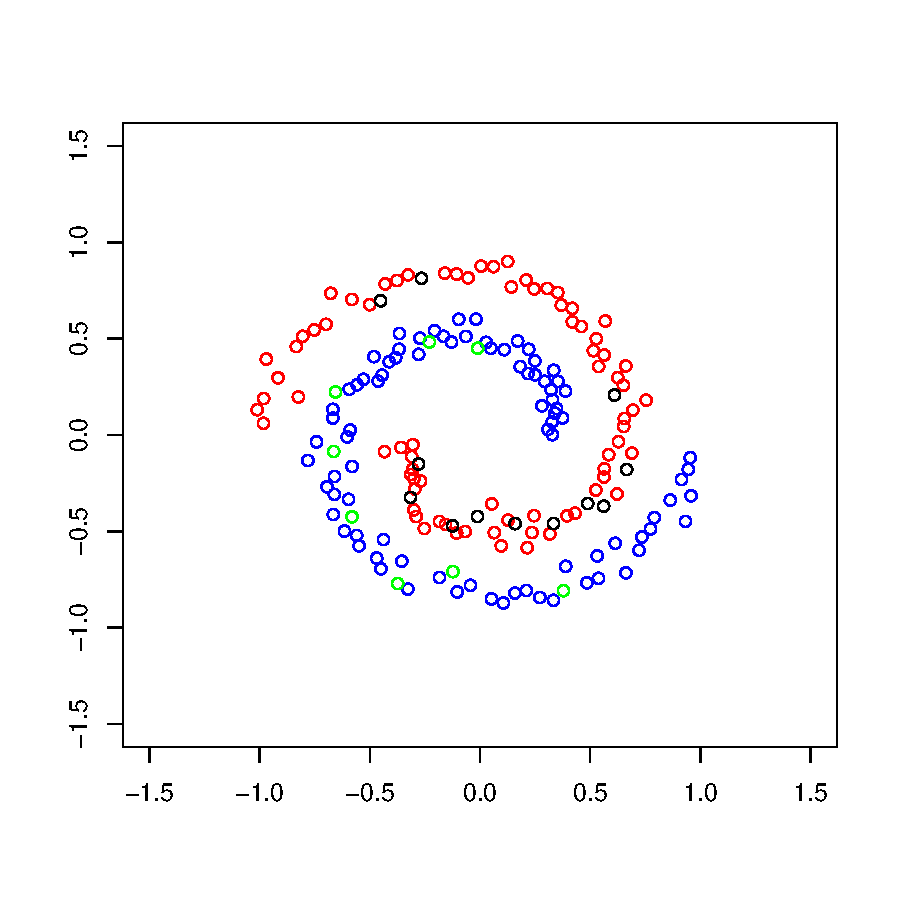
\includegraphics{KDE-007}
\caption{Amostras após a classificação para o fold 1. Em pretro as amostras classificadas como vermelho e em verde as amostras classificadas com azul. }
\label{10}
\end{figure}

\section{Discussão}

  \par Os gráficos das amostras antes e depois da ilustração foram interessantes para ilustrar a capacidade de classificação do nosso algoritmo. Como a espiral está muito bem comportada, somos capazes de ver se a classificação ocorreu conforme o esperado.
  
  \par Além disso, com o gráfico da superfície de densidade de probabilidade podemos observar os contornos das funções de densidade de verossimilhanças estimadas pelo método KDE. Podemos notar que esses contornos seguem o formato espiral das duas classes e resultam na separação linear das classes, como pode ser observado no gráfico dos dados de teste no espaço das verossimilhanças. Nota-se, portanto, que a técnica adotada fez com que um problema de separação não-linear no espaço dos atributos se tornasse linear no espaço das verossimilhanças, o que possibilita a sua classificação.
  
   \par Com o experimento foi possível compreender melhor o funcionamento do classificador de Bayes com o KDE e implementá-lo de forma satisfatória. Os resultados obtidos podem provar que o classificador de Bayes com o KDE mostrou-se muito eficiente para esse conjunto de dados. 
%%%%%%%%%%%%%%%%%%%%%%%%%%%%%%%%%%%%%%%%%%%%%%%%%%%%%%%%%%%%%%%%%%%%%%%%%%%%%%%%%%%%%%%%%

%%%%%%%%%%%%%%%%%%%%%%%%%%%%%%%%%%%%%%%%%%%%%%%%%%%%%%%%%%%%%%%%%%%%%%%%%%%%%%%%%%%%%%%%%


\end{document}
